\section{Технические аспекты}
\subsection{Архитектура программного комплекса}
Современные стандарты языка С++, основанные на так называемом метапрограммировании (использовании шаблонов) позволяют достичь высокой абстракции при программировании различных задач и, как следствие, высокой повторной используемости кода \cite{alexandrescu}. Причём это минимально отражается на производительности программы, в отличие от более распространённого в других объектно-ориентированных языках механизма виртуальных функций.

Программный комплекс был реализован с учётом этих стандартов, благодаря чему допускает расширение на произвольные численные методы, модели механики сплошной среды и и типы материалов. Это иллюстрируют следующие uml-диаграммы компонентов комплекса.

Расчётная сетка \ref{pic:uml-mesh} и численные алгоритмы \ref{pic:uml-gcm} шаблонизированы по типу математической модели сплошной среды, топологии расчётной сетки и типу материала. Благодаря этому при всём многообразии моделей, структурированных и неструктурированных расчётных сеток и типов материалов для реализации новой функциональности программы необходимо дописать только ту часть кода, которая ответственна именно за эту функциональность.

\begin{figure}[H]
	\center{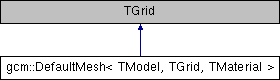
\includegraphics[width=0.6\textwidth]{png/uml/mesh.png}}
	\caption{Архитектура класса расчётной сетки}
	\label{pic:uml-mesh}
\end{figure}

\begin{figure}[H]
	\center{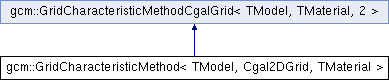
\includegraphics[width=0.8\textwidth]{png/uml/gcm.png}}
	\caption{Архитектура класса численного метода на неструктурированной расчётной сетке}
	\label{pic:uml-gcm}
\end{figure}

Ещё одним полезным инструментом является реализованная библиотека линейной алгебры для работы с матрицами и векторами небольшой размерности. Использование по всему коду её основного класса -- матрицы и вектора (рис. \ref{pic:uml-linal}) -- с определёнными для них функциями и операторами позволяет существенно упростить запись многих алгоритмов и снизить вероятность ошибок при их программировании без существенных потерь в производительности.

\begin{figure}[H]
	\center{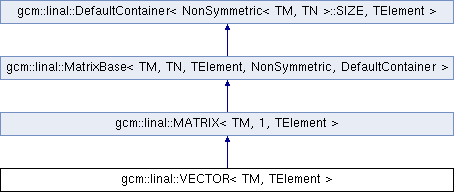
\includegraphics[width=0.9\textwidth]{png/uml/linal.png}}
	\caption{Архитектура базового класса локальной библиотеки линейной алгебры}
	\label{pic:uml-linal}
\end{figure}

Отдельно стоит обратить внимание на используемую в программе для построения и хранения неструктурированной расчётной сетки библиотеку CGAL - Computational geometry algorithms \cite{cgal}, которая также основана на упомянутых выше принципах программирования и является очень полезным инструментом для работы со сложными геометрическими задачами.

\subsection{Параллельность расчётов}
Для возможности проведения расчётов с высокой точностью необходима реализация параллельных алгоритмов выполнения программы. Относительная простота распараллеливания расчётов является сильной стороной явных численных методов, к которым принадлежит сеточно\hyp{}характеристический.

В данной работе был реализован параллельный расчёт с раздельной памятью (MPI) для структурированных сеток и параллельный расчёт с общей памятью (OpenMP) для неструктурированных сеток. На рис. \ref{pic:mpi-perf} и \ref{pic:omp-perf} показаны графики времени выполнения тестовых расчётов (a) c выводом на жёсткий диск рассчитанных данных на каждом временном слое, (b) без вывода данных на жёсткий диск, (с) относительное ускорение в случае (a), (d) относительное ускорение в случае (b). Расчёты выполнялись на современном персональном компьютере с шестиядерным процессором (12 виртуальных ядер).

Анализ графиков показывает фактическую независимость ускорения MPI от вывода данных, что объясняется тем, что вывод данных на жёсткий диск в системе с раздельной памятью также происходит параллельно (тут стоит отметить, что такая закономерность на персональном компьютере нарушится, если программа займёт большую часть памяти системы). 

На неструктурированных сетках с OpenMP вывод данных был реализован в один поток, что, как видно из графиков, привело к значительному снижению эффективности распараллеливания. Также в случае неструктурированных сеток значительное время занимает построение расчётной сетки в начале расчёта. Можно сделать следующие выводы: в случае общей памяти необходимо выделение дампа данных в отдельные потоки исполнения и использование многопоточного алгоритма построения сетки.

\begin{figure}[H]
	\center{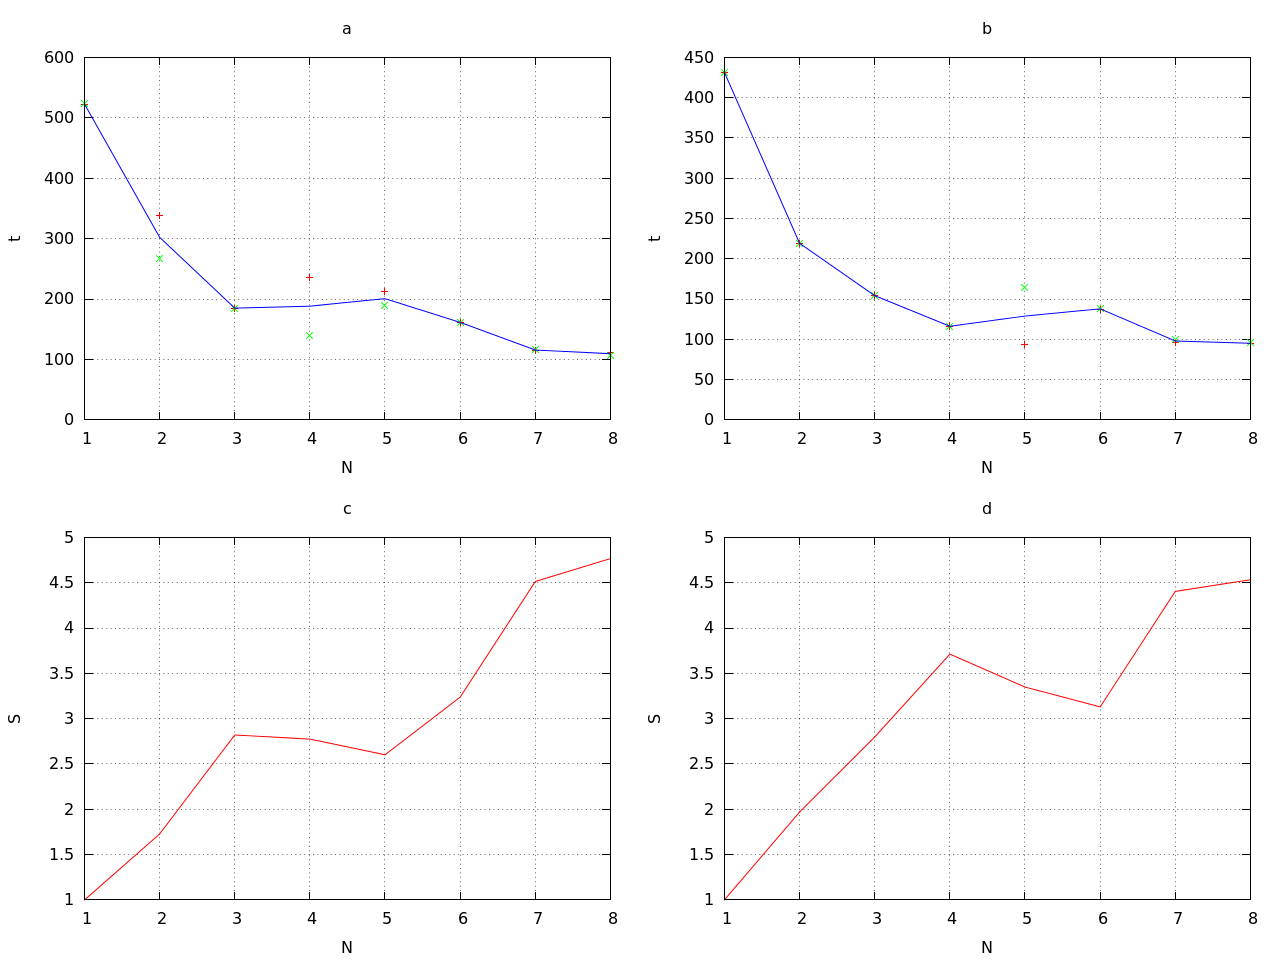
\includegraphics[width=0.8\textwidth]{png/speedup/mpi-perf.png}}
	\caption{Ускорение расчётов на структурированной сетке с использованием MPI}
	\label{pic:mpi-perf}
\end{figure}

\begin{figure}[H]
	\center{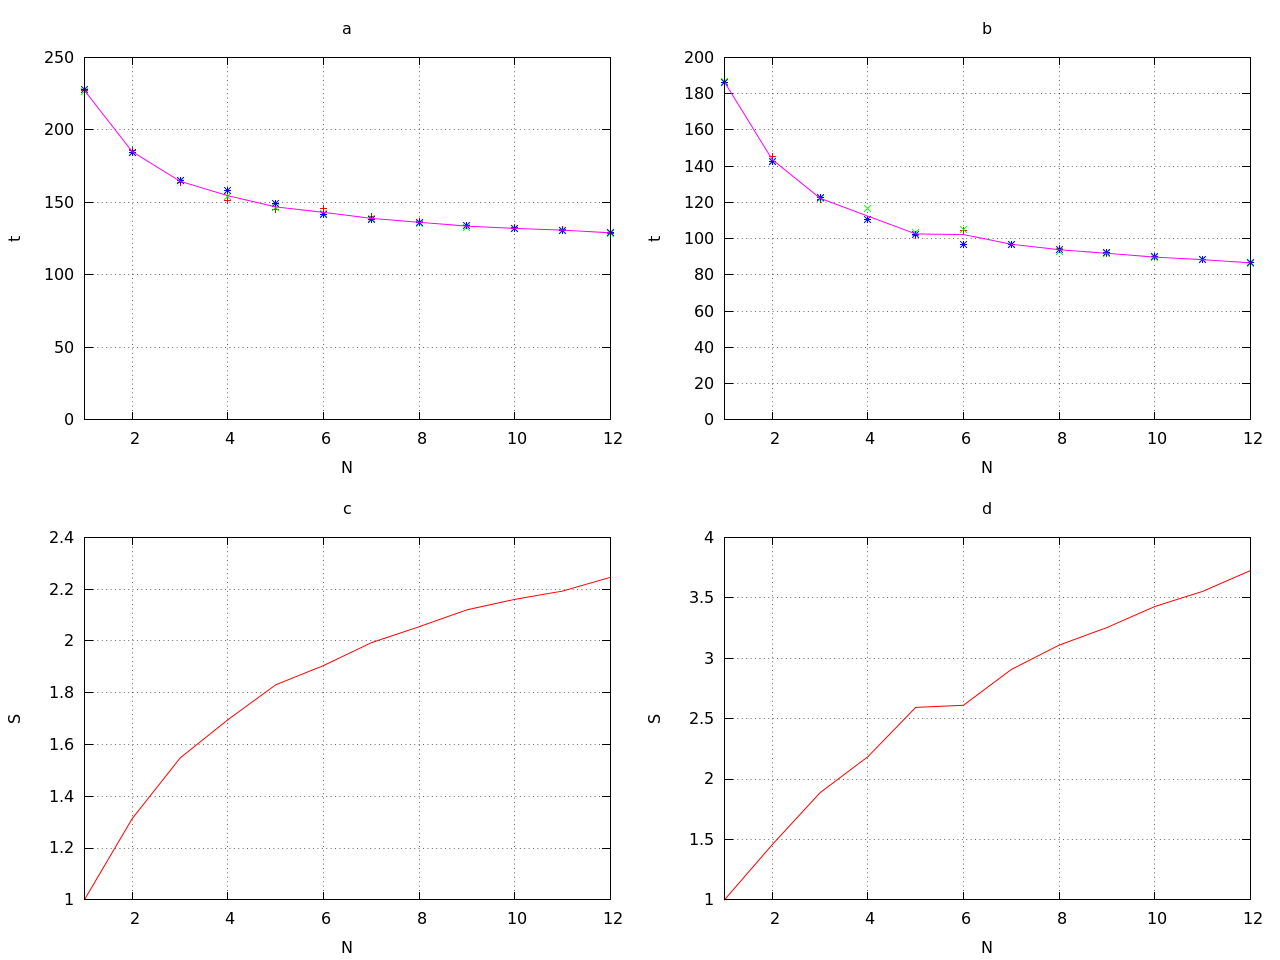
\includegraphics[width=0.8\textwidth]{png/speedup/omp-perf.png}}
	\caption{Ускорение расчётов на неструктурированной сетке с использованием OpenMP}
	\label{pic:omp-perf}
\end{figure}


















